\documentclass[a5 paper, 11pt]{article}
\usepackage[utf8]{inputenc}
\usepackage[lmargin=3cm,rmargin=2.5cm,tmargin=2cm,bmargin=2cm]{geometry}
\usepackage{multicol}
\usepackage{xcolor}
\usepackage{float}
\usepackage{graphicx}
\usepackage{dirtytalk}
\usepackage[export]{adjustbox}
\usepackage{fancyhdr}
\pagestyle{fancy}
\fancyhf{}
\rhead{Adrian Archundia Juarez}
\lfoot{\leftmark}
\cfoot{\thepage}
\pagecolor{brown}
\title{Una aventura extraordinaria}
\author{adrianarch }
\date{September 2022}

\begin{document}
\begin{center}

\Huge{\textbf{Una aventura extraoridinaria}}\\
\huge{Computación 8180\\
September 2022}
\end{center}


\section{Reseña}
Después de decidir vender su zoológico en la India y mudarse a Canadá, Santosh y Gita Patel viajan en un barco carguero con sus hijos y algunos animales. Una terrible tormenta hunde el barco, dejando a Pi, el hijo de los Patel, como el único sobreviviente humano. Sin embargo, Pi no está solo; un temible tigre de bengala lo acompaña en el bote salvavidas. Los días se vuelven semanas y meses, y Pi y el tigre deben aprender a confiar el uno en el otro para sobrevivir.

\section{Reparto}
\begin{multicols}{2}
\begin{enumerate}
    \item \fcolorbox{yellow}{red}{\textcolor{green}{Suraj Sharma como Pi Patel}}
    \item \fcolorbox{yellow}{red}{\textcolor{green}{Irrfan Khan como Pi Patel (adulto)}}
    \item \fcolorbox{yellow}{red}{\textcolor{green}{Tabu como Gita Patel}} 
    \item Gautam Belur
    \item Vibish Sivakumar
    \item Gerard Depardieu
    \newpage
    \item Adil Hussain 
    \item Rafe Spall
    \item Ayush Tandon
    \item Ayaan Khan
    \item Shravanthi Sainath
    \item Abbas Khaleeli
    \item Andrea Di Stefano
    \item James Saito
    \item Jun Naito
    \item Huang Jian-Wei
    \item Wang Bo Chieh
    \item Elie Alouf
    \item Karthik
    \item Amarendran Ramanan
    \item Mythili Prakash
    \item Ko I-Chen
    \item Iswar Srikumar
    \item Nitya Mehra
    \item Bombay Jayashri
    \item Pondy Ravi
    \item Dean Georgaris
    \item Navi Dhanoa

\end{enumerate}
\end{multicols}

\textcolor{red}{Se puede ver el lugar y el contexto en donde se desarrolla la trama}
\begin{figure}[H]
    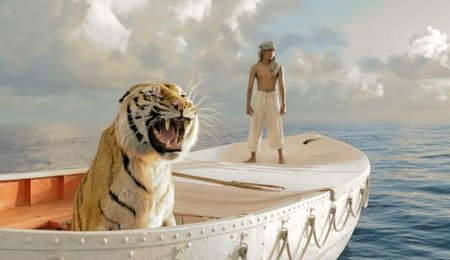
\includegraphics[scale=0.4,angle=15,right]{pi.jpg}
  
\end{figure}

\section{¿Porque Pi?}
\textcolor{red}{Porque muestra los limites del ser humano cuando se tarta de sobrevivir.}\\
\textcolor{green}{Otro punto a toma es que se nos enseña que el trabajo en equipo siempre beneficia cuando se sabe colaborar y sin importar el compañero.}\\
\textcolor{blue}{y por ultimo es muy ineteresante ver como se desarrolla un personaje en una situacion de vulnerabilidad en todo momento.}\\

\begin{figure}[H]
    \centering
    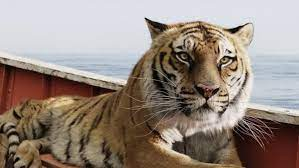
\includegraphics[scale=0.50,rotate=-18]{r parker.jpg}
    \caption{Richard Parker en la barca en donde se desarrolla la historia}
    
\end{figure}
\begin{figure}[H]
    \centering
    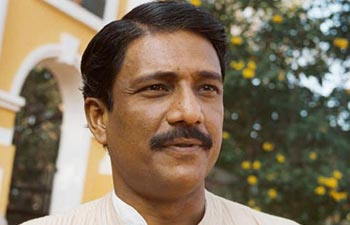
\includegraphics[scale=0.50,rotate=8]{papa pi.jpg}
    \caption{El padre de pi quien fue el que decidio que la familia tome el viaje en donde Pi quedo naufrago}
    
\end{figure}
\hspace{-2cm}\say{{Las cosas no salieron}

\hspace{-2cm}{como debieron, pero}

\hspace{-2cm}{¿Que se le va a hacer?}

\hspace{-2cm}{hay que acerptar la vida}

\hspace{-2cm}{como venga y sacarle}

\hspace{-2cm}{el mejor partido posible}}
\end{document}
